\chapter{GIỚI THIỆU}
\label{Chapter1}
%
Chương này nhằm giới thiệu tổng quan về đề tài phát hiện hình ảnh tạo sinh, một vấn đề nổi bật trong lĩnh vực thị giác máy tính hiện đại. Mở đầu chương trình bày bối cảnh và vấn đề nghiên cứu trong bối cảnh sự phát triển nhanh chóng của các mô hình tạo sinh ảnh như GAN~\cite{Goodfellow2014GenerativeAN} và Diffusion~\cite{Ho2020DenoisingDP}. Tiếp theo, chương làm rõ động lực nghiên cứu cả về mặt khoa học và ứng dụng thực tiễn, từ đó xác lập mục tiêu nghiên cứu, phát biểu hình thức của bài toán, các thách thức kỹ thuật cần giải quyết, và phạm vi triển khai. Cuối cùng, chương trình bày những đóng góp chính của luận văn như một nền tảng định hướng cho các chương tiếp theo.
%
\section{Bối cảnh và vấn đề nghiên cứu}

Sự phát triển vượt bậc của trí tuệ nhân tạo, đặc biệt trong lĩnh vực học sâu, đã thúc đẩy sự ra đời của các mô hình tạo sinh hình ảnh ngày càng tinh vi và chính xác. Những mô hình như Generative Adversarial Networks~\cite{Goodfellow2014GenerativeAN} và Diffusion~\cite{Ho2020DenoisingDP} có khả năng tạo ra hình ảnh có chất lượng gần như tương đương với hình ảnh thật, gây khó khăn đáng kể trong việc phân biệt bằng mắt thường. Đây vừa là một bước tiến đột phá trong công nghệ xử lý ảnh, vừa đặt ra những thách thức lớn về mặt nhận diện, xác thực và quản lý thông tin.

Vấn đề đặt ra là: khi ranh giới giữa ảnh thật và ảnh giả ngày càng trở nên mờ nhạt, làm thế nào để các hệ thống tự động có thể phân biệt chính xác hình ảnh do con người chụp với hình ảnh do máy sinh ra? Câu hỏi này đặc biệt cấp thiết trong bối cảnh ảnh tạo sinh có thể bị lợi dụng để phát tán thông tin sai lệch, giả mạo nhân thân, hoặc phục vụ các mục đích phi đạo đức và phi pháp khác.

Từ đó, bài toán phát hiện hình ảnh tạo sinh trở thành một hướng nghiên cứu quan trọng và mang tính thời sự cao. Luận văn này tập trung vào việc phân tích, đánh giá và đề xuất phương pháp phát hiện ảnh tạo sinh, nhằm góp phần vào nỗ lực xây dựng các hệ thống nhận diện hình ảnh tin cậy, đáp ứng cả yêu cầu học thuật lẫn ứng dụng thực tiễn trong bối cảnh phát triển nhanh của công nghệ tạo sinh hình ảnh.
%
\section{Động lực nghiên cứu}
%
\subsection{Động lực khoa học}
Phát hiện hình ảnh tạo sinh là một trong những nhiệm vụ khó khăn trong lĩnh vực thị giác máy tính, nhiệm vụ này đặt trọng tâm vào việc phân tích và nhận diện các đặc điểm không tự nhiên trong ảnh – những dấu hiệu có thể chỉ ra sự can thiệp của các mô hình tổng hợp ảnh. 
%
%Các dấu hiệu giả mạo này ngày càng khó phát hiện được bằng mắt thường do sự phát triển nhanh và mạnh mẽ của các mô hình tạo sinh ảnh. Dưới góc nhìn khoa học, nhiệm vụ này có ý nghĩa quan trọng.
%

Sự phát triển nhanh chóng của các mô hình tạo sinh ảnh, đặc biệt là GANs~\cite{Goodfellow2014GenerativeAN} và Diffusion Models~\cite{Ho2020DenoisingDP}, đã tạo ra một lớp hình ảnh giả có mức độ chân thực ngày càng cao. Điều này đặt ra nhu cầu cấp thiết cho cộng đồng nghiên cứu trong việc phát triển các phương pháp phát hiện ngày càng tinh vi hơn, có khả năng thích ứng với sự thay đổi liên tục của các kỹ thuật tạo sinh.
%

Từ góc nhìn khoa học, việc nghiên cứu phát hiện hình ảnh tạo sinh không chỉ giúp nâng cao hiểu biết về cấu trúc và tính chất của dữ liệu hình ảnh, mà còn góp phần vào việc phát triển các mô hình học sâu có khả năng khái quát tốt hơn. Một thách thức lớn hiện nay là hầu hết các phương pháp phát hiện chỉ hoạt động hiệu quả trên ảnh được tạo ra từ những mô hình tương tự với mô hình đã thấy trong giai đoạn huấn luyện. Do đó, việc đề xuất các phương pháp phát hiện có tính tổng quát cao là một vấn đề khoa học quan trọng, có thể thúc đẩy sự hiểu biết sâu sắc hơn về mối quan hệ giữa mô hình sinh và đặc trưng ảnh.
%
%Với tiềm năng ứng dụng rộng lớn trong nhiều lĩnh vực, ngay cả trong lĩnh vực yêu cầu độ tin cậy cao như y tế, được phẩm \cite{wolleb2022diffusionmodelsmedicalanomaly,kazerouni2023diffusionmodelsmedicalimage}, các công nghệ tạo sinh hình ảnh như Generative Adversarial Networks (GANs)~\cite{Goodfellow2014GenerativeAN} , Diffusion~\cite{Ho2020DenoisingDP} đang thu hút sự đầu tư mạnh mẽ từ xã hội nhằm không ngừng cải thiện, nâng cao chất lượng. Việc phát hiện hình ảnh giả mạo cung cấp những phản hồi quan trọng để cải thiện chất lượng những mô hình này \cite{Ho2020DenoisingDP, Goodfellow2014GenerativeAN} giúp chúng ngày càng trở nên hoàn hảo, tin cậy.

%Bên cạnh những tiến bộ đáng kể trong việc phát triển các phương pháp phát hiện giả mạo \textcolor{red}{(Chèn bảng hoặc chart cho thấy quá trình phát triển) }, nhược điểm lớn nhất ở những phương pháp hiện nay là chúng hoạt động hiệu quả khi hình ảnh tạo sinh đến từ các mô hình có kiến trúc giống hoặc tương tự với mô hình đã sử dụng để sinh dữ liệu trong quá trình huấn luyện, nhưng lại không ổn định khi áp dụng cho hình ảnh sinh từ các mô hình mới, do đó cần phải phát triển những phương pháp mới, song song với sự phát triển của các mô hình tạo sinh.

Tóm lại, việc nghiên cứu và hoàn thiện các phương pháp phát hiện ảnh giả mạo không chỉ góp phần nâng cao tính minh bạch và độ tin cậy của công nghệ tạo sinh hình ảnh, mà còn đóng vai trò quan trọng trong việc đảm bảo an toàn thông tin và bảo vệ hệ thống thị giác máy tính trước các nguy cơ giả mạo.

%\subsection{Động lực ứng dụng}
%Trong những năm gần đây, các mô hình tạo sinh ảnh đã có những bước tiến dài, và đã có những ứng dụng tích cực vào cuộc sống. Nổi trội trong các mô hình tạo sinh ảnh là Generative Adversarial Networks \cite{Goodfellow2014GenerativeAN} (GANs) và Diffusion \cite{Ho2020DenoisingDP}, trong đó các phiên bản của mô hình Diffusion có hiệu suất đáng kinh ngạc với khả năng sinh ra hình ảnh chất lượng cao và giống với hình ảnh thực tế như Stable Diffusion 3~\cite{Esser2024ScalingRF} và một số nền tảng phố biến hiện nay như  DALL-E~\cite{dalle2}, DeepArt~\cite{deepart} cũng đang là công cụ hổ trợ mạnh mẽ trong nhiều lĩnh vực như thiết kế đồ hoạ \cite{CasteleiroPitrez2024GenerativeAI,Shin2024CanPM}, thời trang \cite{8769486}, nội thất \cite{Chen2020ApplicationOA}, sáng tác nghệ thuật \cite{Ai_won_an_art_contest}. 
%
%Tuy nhiên bên cạnh những ứng dụng hữu ích cũng xuất hiện những ứng dụng tiêu cực từ công nghệ này \cite{DBLP-abs-2107-10139}, các hình ảnh giả mạo, gây hiểu lầm phục vụ cho nhiều mục đích xấu khác nhau như lừa đảo \cite{Ai_chief_financial_officer}, bôi nhọ danh dự cá nhân \cite{VirginiaDeepfake}, tình trạng này dẫn đến một số nơi trên thế giới đã áp dụng các chế tài ngăn chặn \cite{CaliforniaDeepfakes}. Chất lượng các mô hình tạo sinh ảnh ngày càng nâng cao, việc nhận biết một hình ảnh là do mô hình tạo sinh (ảnh giả) bằng mắt thường dần trở nên khó khăn \cite{spottingai}. 
%
%Tiếp cận và sử dụng các công cụ trí tuệ nhân tạo để sinh ra hình ảnh giả rất đơn giản, số lượng hình ảnh sinh ra trong một ngày cũng là một con số khổng lồ, vì vậy cần có giải pháp phát hiện, xác minh một hình ảnh là thật hay giả hiệu quả và tự động. Hơn nữa, sự gia tăng sử dụng các thiết bị thông minh như điện thoại thông minh và máy tính bảng đã tạo điều kiện thuận lợi cho việc phát tán hình ảnh và thông tin giả mạo trên quy mô lớn. Do đó, cần thiết phải phát triển các phương pháp xác minh tính xác thực của thông tin một cách nhanh chóng, có thể được triển khai ngay trên những thiết bị có cấu hình thấp và tài nguyên hạn chế.
%%

\subsection{Động lực ứng dụng}

Trong những năm gần đây, các mô hình tạo sinh hình ảnh đã có những bước tiến vượt bậc và được ứng dụng rộng rãi trong thực tiễn. Nổi bật trong số đó là các mô hình Generative Adversarial Networks (GANs)~\cite{Goodfellow2014GenerativeAN} và Diffusion~\cite{Ho2020DenoisingDP}, đặc biệt là các phiên bản mới như Stable Diffusion 3~\cite{Esser2024ScalingRF}. Các mô hình này có khả năng sinh ra hình ảnh chất lượng cao, gần giống ảnh thật đến mức khó phân biệt bằng mắt thường.

Các nền tảng ứng dụng như DALL-E~\cite{dalle2}, DeepArt~\cite{deepart} hiện đang được sử dụng hiệu quả trong nhiều lĩnh vực như thiết kế đồ họa~\cite{CasteleiroPitrez2024GenerativeAI,Shin2024CanPM}, thời trang~\cite{8769486}, nội thất~\cite{Chen2020ApplicationOA}, và sáng tác nghệ thuật~\cite{Ai_won_an_art_contest}, mang lại những giá trị sáng tạo và hiệu quả vượt trội.

Tuy nhiên, song song với các ứng dụng tích cực, công nghệ này cũng bị lợi dụng cho những mục đích tiêu cực~\cite{DBLP-abs-2107-10139}, chẳng hạn như tạo ra hình ảnh giả để lừa đảo~\cite{Ai_chief_financial_officer}, bôi nhọ danh dự cá nhân~\cite{VirginiaDeepfake}, hoặc thao túng dư luận. Trước thực trạng này, một số quốc gia đã ban hành các quy định và chế tài để kiểm soát việc phát tán hình ảnh giả mạo~\cite{CaliforniaDeepfakes}.

Chất lượng hình ảnh do các mô hình tạo sinh tạo ra ngày càng tinh vi khiến việc phân biệt ảnh thật và ảnh giả bằng mắt thường trở nên khó khăn~\cite{spottingai}. Hơn nữa, việc tiếp cận và sử dụng các công cụ AI tạo ảnh hiện nay rất đơn giản, cho phép bất kỳ ai cũng có thể tạo ra số lượng lớn hình ảnh giả chỉ trong thời gian ngắn.

Trong bối cảnh đó, việc phát triển các giải pháp có khả năng phát hiện và xác minh hình ảnh giả một cách hiệu quả và tự động là hết sức cần thiết. Đặc biệt, các giải pháp này cần đảm bảo khả năng triển khai trên những thiết bị phổ thông như điện thoại thông minh hoặc máy tính bảng, vốn có tài nguyên phần cứng hạn chế, nhằm hạn chế sự lan truyền của thông tin sai lệch trên quy mô lớn.


\section{Mục tiêu nghiên cứu}
Phát triển phương pháp phân biệt ảnh tạo sinh đạt được hai mục tiêu sau:
\begin{itemize}
	\item Phương pháp có hiệu quả trên nhiều loại mô hình tạo sinh khác nhau
	\item Yêu cầu sức mạnh tính toán và lưu trữ thấp, tốc độ nhanh, phù hợp triển khai trên những thiết bị có cấu hình, tài nguyên hạn chế.
\end{itemize}

\section{Phát biểu bài toán}
%
\subsection{Định nghĩa về Ảnh Thật và Ảnh Tạo Sinh}
Trong khuôn khổ của đề tài, ta định nghĩa và phân biệt hai loại hình ảnh (2 lớp đối tượng) của bài toán:
\begin{itemize}  

    \item \textbf{Ảnh Tạo Sinh (ảnh giả mạo)}: Là những hình ảnh được tạo ra bởi mô hình GAN~\cite{Goodfellow2014GenerativeAN}, mô hình Diffusion \cite{Ho2020DenoisingDP}, hoặc bất kỳ mô hình tạo sinh khác. Nôi dung của hình ảnh tạo sinh là mô phỏng theo các đối tượng từ thế giới thật hoặc có thể là một đối tượng mới không có thật.
    
    \item \textbf{Ảnh Thật}: Là những hình ảnh được chụp từ thực tế bằng máy ảnh hoặc các thiết bị thu hình khác. Những hình ảnh này phản ảnh chân thực các đối tượng của thế giới thực, bao gồm cả ảnh chụp các tác phẩm nghệ thuật, hoặc ảnh chụp lại một hình ảnh tạo sinh.

\end{itemize}
%
\subsection{Phát biểu hình thức}
%
Phát hiện hình ảnh tạo sinh là bài toán xác định một hình ảnh là \textit{ảnh thật} được tạo ra bằng thiết bị thu hình như máy ảnh, máy quay phim, hay \textit{ảnh tạo sinh} được tạo ra bằng cách sử dụng các mô hình tạo sinh như GAN~\cite{Goodfellow2014GenerativeAN} hoặc Diffusion~\cite{Ho2020DenoisingDP}. Trong luận văn này, bài toán phát hiện hình ảnh tạo sinh được định hình như một bài toán phân loại trong lĩnh vực thị giác máy tính và được mô tả cụ thể như sau:\\
%
\textbf{Đầu vào:} Ảnh đầu vào $I \in \mathbb{R}^{w \times h \times c}$, trong đó $w ,h, c$ tương ứng chiều rộng, chiều cao và số lượng kênh màu của hình ảnh.\\
%
\textbf{Đầu ra: } Là kết quả dự đoán thể hiện ảnh đầu vào $I$ là ảnh thật hay ảnh giả mạo.
\begin{equation}
y = f(I)
\end{equation}
Với  \( y \in \{0, 1\} \) là nhãn phân loại của ảnh \( I \), $f(.)$ là bộ phân loại.
\begin{itemize}
    \item Nếu \( y = 0 \), thì \( I \) được phân loại là ảnh thật.
    \item Nếu \( y = 1 \), thì \( I \) được phân loại là ảnh tạo sinh.
\end{itemize}
%
%
\subsection{Phương pháp giải bài toán}

Bài toán phát hiện hình ảnh tạo sinh được tiếp cận dưới dạng bài toán phân loại nhị phân, trong đó mô hình học sâu cần phân biệt giữa ảnh thật (do máy ảnh chụp) và ảnh giả (được sinh ra bởi các mô hình tạo sinh như GAN~\cite{Goodfellow2014GenerativeAN} hoặc Diffusion~\cite{Ho2020DenoisingDP}). Phương pháp được đề xuất trong luận văn gồm hai giai đoạn chính: \textbf{tiền xử lý ảnh đầu vào} và \textbf{huấn luyện bộ phân lớp học sâu.}

Trước khi đưa ảnh vào mô hình học sâu, ảnh đầu vào được xử lý bởi một bộ lọc tần số cao trong miền không gian. Bộ lọc này được thiết kế nhằm làm nổi bật các chi tiết vi mô hoặc những nhiễu đặc trưng mà các mô hình tạo sinh thường để lại. Thay vì sử dụng trực tiếp \gls{fft}~\cite{Arunachalam2013TheFF} – vốn yêu cầu chuyển đổi qua lại giữa miền không gian và miền tần số, luận văn đề xuất một bộ lọc tương đương trong miền không gian có tên gọi là \textbf{ADOF}. Cụ thể, bộ lọc được xây dựng bằng cách thiết kế một \gls{kernel} với đáp ứng tương tự bộ lọc thông cao, cho phép loại bỏ các thành phần tần số thấp và giữ lại các chi tiết tần số cao vốn dễ thể hiện sự khác biệt giữa ảnh thật và ảnh giả.

Ảnh sau khi được lọc sẽ giữ lại nhiều đặc trưng hữu ích cho quá trình học, đồng thời giảm nhiễu từ nền ảnh hoặc cấu trúc toàn cục. Đây là bước quan trọng giúp tăng độ nhạy của mô hình đối với các tín hiệu tinh vi mà ảnh tạo sinh thường để lộ.

Sau bước tiền xử lý, ảnh được đưa vào mô hình học sâu \( f(\cdot) \) - một hàm phân lớp có đầu vào là ảnh đã xử lý và đầu ra là xác suất ảnh thuộc lớp giả mạo. Các bước cụ thể được mô tả như sau:
\[
\mathbf{x}_i^{\text{filtered}} = \mathcal{F}(\mathbf{x}_i), \quad \hat{y}_i = f(\mathbf{x}_i^{\text{filtered}})
\]
Trong đó,
\(\mathbf{x}_i^{\text{filtered}}\) là hình ảnh sau khi áp dụng bộ lọc thông cao,
\( \mathcal{F}(\cdot) \) là phép lọc không gian tương đương với lọc thông cao mà luận văn xây dựng,
\( \mathbf{x}_i \) là ảnh gốc, và \( \hat{y}_i \in [0,1] \) là xác suất đầu ra.

Quá trình huấn luyện nhằm tìm bộ tham số \( \theta \) của mô hình sao cho hàm mất mát cross-entropy~\cite{2023arXiv230407288M} đạt giá trị nhỏ nhất:
\[
\hat{\theta} = \arg \min_{\theta} \mathcal{L}(\theta)
\]
Với hàm mất mát:
\[
\mathcal{L}(\theta) = -\frac{1}{N} \sum_{i=1}^{N} \left[ y_i \log(\hat{y}_i) + (1 - y_i) \log(1 - \hat{y}_i) \right]
\]
Trong đó:
\begin{itemize}
	\item \( N \): số lượng mẫu huấn luyện,
	\item \( y_i \in \{0, 1\} \): nhãn thực tế, với 0 là ảnh thật và 1 là ảnh giả,
	\item \( \hat{y}_i = f(\mathcal{F}(\mathbf{x}_i)) \): xác suất mô hình dự đoán ảnh là giả sau tiền xử lý.
\end{itemize}

Việc kết hợp kỹ thuật tiền xử lý với mô hình học sâu giúp khai thác được cả đặc trưng miền không gian và đặc trưng tần số, từ đó nâng cao khả năng phát hiện ảnh tạo sinh, đặc biệt trong các trường hợp khó nhận biết bằng mắt thường.

%
\section{Thách thức bài toán}

Tốc độ phát triển của công nghệ tạo ảnh bằng mạng học sâu làm cho các phương pháp phân biệt giữa ảnh thật và ảnh giả mạo nhanh chóng lỗi thời, kém hiệu quả trên các mô hình tạo sinh mới:

\begin{itemize}
	\item Khó khăn với nhóm phương pháp phát hiện ảnh giả mạo dựa trên sự không đồng nhất ở cấp độ ngữ nghĩa hình ảnh: Hướng tiếp cận này dựa vào việc phát hiện các bất hợp lý về ngữ nghĩa, màu sắc, hình dạng, hoặc những điểm mâu thuẫn với quy luật vật lý của đối tượng, trong các hình ảnh tạo sinh. Tuy nhiên, chất lượng hình ảnh tạo sinh hiện nay đã được nâng cao đáng kể so với những ngày đầu, làm cho việc áp dụng phương pháp này trở nên ngày càng khó khăn hơn (Hình~\ref{fig:ai-real-samples-1b}).
	\begin{figure}[htp]
		\centering
		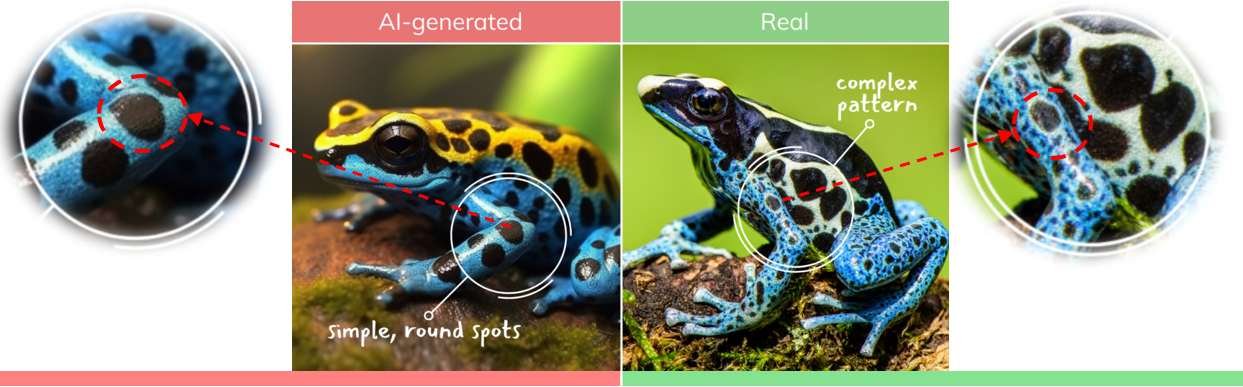
\includegraphics[width=0.9\linewidth]{ai-real-samples-1b.png}
		\begin{minipage}{0.9\linewidth}
			\caption{Ảnh tạo sinh \textit{(trái)} và ảnh thật \textit{(phải)}, được phân biệt dựa vào mức độ chi tiết trên hoa văn của đối tượng. \textit{Nguồn: \url{https://elearn.eb.com}}}
			\label{fig:ai-real-samples-1b}
		\end{minipage}
	\end{figure}\\
	%
	Bênh cạnh đó để huấn luyện mô hình \textit{"hiểu"} được các điểm bất hợp lý là bài toán khó, yêu cầu dữ liệu huấn luyện lớn và việc gán nhãn vị trí bất hợp lý trên hình ảnh cần nhiều chi phí, vì vậy hướng tiếp cận này ít được sử dụng hiện nay, tuy nhiên đây có thể là hướng phát triển tiềm năng khi kết hợp với mô hình ngôn ngữ lớn vì nó cho đưa ra được giải thích cho kết quả dự đoán.
	%
	\item Phát hiện hình ảnh giả mạo dựa vào phân tích, rút trích các đặc trưng tần số hay đặc trưng không gian trên hình ảnh. Hướng tiếp cận này mặc dù đem lại kết quả cao, ít phụ thuộc vào ngữ nghĩa của hình ảnh, tuy nhiên các kiến trúc mô hình khác nhau sẽ tạo ra những dấu vết khác nhau, do đó, thách thức lớn trong việc tìm ra đặt trưng chung và có hiệu quả trên nhiều mô hình tạo sinh (Hình~\ref{fig:gan-fingerprints-1}).
	
	\begin{figure}[h]
		\centering
		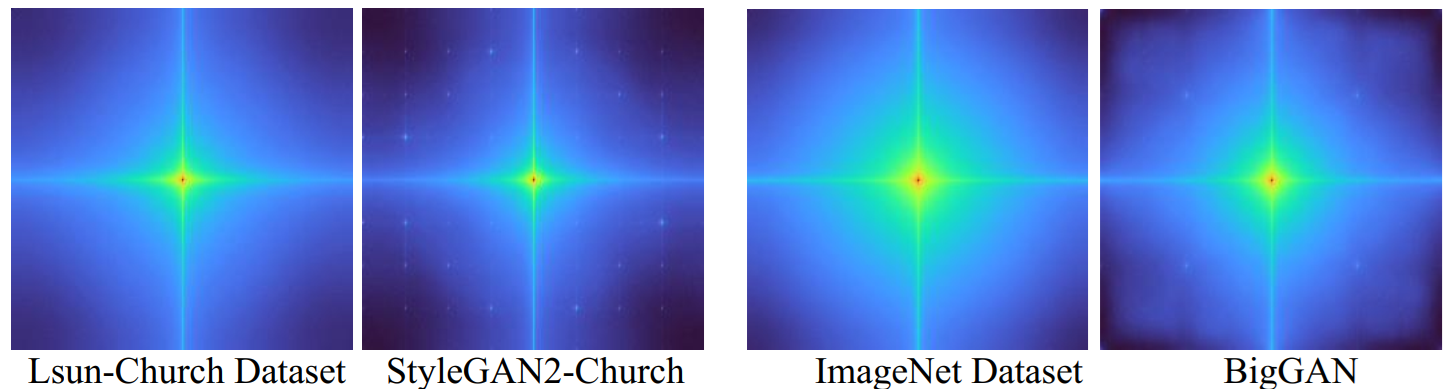
\includegraphics[width=1.0\textwidth]{gan-fingerprints-1.png}
	    \vspace{10pt} % Thay đổi khoảng cách giữa ảnh và chú thích
	    
		\begin{minipage}{\linewidth}
			\caption{Trung bình phổ Fourier của 2,000 hình ảnh từ tập dữ liệu Lsun \textit{(trái)} và ImageNet \textit{(phải)}, các dấu vết khác nhau giữa mô hình StyleGAN2 và BigGAN thể hiện ở hình 2 và 4 từ trái sang.}
			\label{fig:gan-fingerprints-1}
		\end{minipage}
	\end{figure}
	%
\end{itemize}
%
Ảnh tạo sinh rất đa dạng về nội dung, hình thức và được tạo ra theo trí tưởng tượng vô hạn của người dùng. Các hướng tiếp cận cho độ chính xác cao hiện nay, đều tận dụng sức mạnh của kỹ thuật học sâu. Tuy nhiên, dữ liệu dùng để huấn luyện các mô hình này không đủ đại diện cho toàn bộ ảnh giả mạo, cụ thể dữ liệu huấn luyện chỉ chứa một số lượng hữu hạn các đối tương trong thế giới thực, nhưng trong thực tế các đối tượng trong ảnh giả mạo có thể nằm ngoài tập huấn luyện, đây là một khó khăn cơ bản của bài toán này.

Khó khăn trong việc trả lời câu hỏi \textit{"mô hình đã dựa vào đâu để đưa ra kết luận?"}, đây là khó khăn chung của việc ứng dụng kỹ thuật học sâu, và trong nhiệm vụ phát hiện ảnh giả mạo thì yêu cầu tính \textit{"giải thích được"} càng quan trọng. Các đặc điểm thể hiện một hình ảnh là giả mạo thường không thể nhận biết một cách trực quan mà là qua sự tổng hợp rút trích đặc trưng của mạng học sâu, do tính chất phức tạp của các mô hình này, việc cung cấp giải thích rõ ràng và minh bạch cho các quyết định của mô hình là một thách thức lớn.

%
\section{Nội dung và phạm vi nghiên cứu}

\subsection{Nội dung nghiên cứu}

Đề tài tập trung vào việc phát hiện hình ảnh tạo sinh bằng cách kết hợp giữa tiền xử lý đặc thù và mô hình học sâu. Các nội dung chính bao gồm:

\begin{itemize}
	\item Khảo sát các mô hình tạo sinh hình ảnh phổ biến như GAN~\cite{Goodfellow2014GenerativeAN} và Diffusion~\cite{Ho2020DenoisingDP}.
	\item Khảo sát các phương pháp phân biệt ảnh thật và ảnh tạo sinh trong miền không gian và miền tần số.
	\item Đề xuất và thiết kế một bộ lọc không gian có chức năng tương đương với bộ lọc thông cao Fourier, nhằm làm nổi bật các đặc trưng giúp phân biệt ảnh giả.
	\item Xây dựng mô hình học sâu \gls{cnn} nhọ gọn để thực hiện phân loại ảnh thật/giả, sử dụng ảnh đầu vào đã được tiền xử lý.
	\item Huấn luyện và đánh giá mô hình trên tập dữ liệu tổng hợp từ nhiều nguồn ảnh thật và ảnh tạo sinh.
\end{itemize}

\subsection{Phạm vi nghiên cứu}

\begin{itemize}
	\item Chỉ tập trung vào ảnh tĩnh (không xử lý video hoặc ảnh động).
	%
	\item Ảnh giả mạo được tạo từ các mô hình tạo sinh phổ biến gồm GAN~\cite{Goodfellow2014GenerativeAN} và Diffusion~\cite{Ho2020DenoisingDP}.
	%
	\item Tập trung và khai thác ưu điểm của các phương pháp tiền xử lý trên miền không gian và miền tần số.
\end{itemize} 
%

\section{Đóng góp của luận văn}
Luận văn có những đóng góp cơ bản sau:
\begin{itemize}
	%
	\item Xây dựng kiến trúc mô hình đơn giản nhưng có hiệu quả cao khi kết hợp với bộ lọc mà luận văn đề xuất. Bộ phân loại sau khi huấn luyện có khả năng hoạt động tốt trên nhiều tập dữ liệu được sinh bởi nhiều loại mô hình tạo sinh khác nhau.
	%
	\item Đề xuất một bộ lọc mới làm tăng độ chính xác của mô hình, tăng tốc độ hội tụ trong quá trình huấn luyện mô hình, đồng thời phương pháp này yêu cầu số lượng phép tính nhỏ hơn nhiều phương pháp khác nhưng vẫn cho độ chính xác cao.
	%
\end{itemize}

\section{Cấu trúc của luận văn}

Luận văn được tổ chức thành 5 chương như sau:

\begin{itemize}
	\item \textbf{Chương 1 – Giới thiệu:} Trình bày bối cảnh, động lực nghiên cứu, mục tiêu, phạm vi và phát biểu bài toán. Chương cũng nêu rõ các thách thức và đóng góp chính của luận văn.
	
	\item \textbf{Chương 2 – Nghiên cứu liên quan:} Tổng quan các mô hình tạo sinh ảnh tiêu biểu và phân tích các nhóm phương pháp phát hiện hình ảnh tạo sinh, bao gồm phương pháp miền không gian, miền tần số và kết hợp.
	
	\item \textbf{Chương 3 – Phương pháp đề xuất:} Mô tả chi tiết quy trình tiền xử lý ảnh, kiến trúc mô hình học sâu, hàm mất mát sử dụng và quy trình huấn luyện mô hình.
	
	\item \textbf{Chương 4 – Thực nghiệm và đánh giá:} Trình bày các tập dữ liệu sử dụng, thiết lập thí nghiệm, các chỉ số đánh giá và kết quả so sánh với các phương pháp khác.
	
	\item \textbf{Chương 5 – Kết luận và hướng phát triển:} Tổng kết các kết quả đạt được và đề xuất một số hướng nghiên cứu mở trong tương lai.
\end{itemize}









